\chapter{Enzymes and Biochemical Catalysis}\label{ch:b1:enzymes}

Pour hydrogen peroxide on a cut potato and it froths: a single molecule
of catalase in the potato's \omterm{def:b1:cell-unit-of-life:cell}{cells} splits forty million molecules of
peroxide every second, a reaction that, left to itself, would take
years. The peroxide was going to decompose anyway --- the reaction is
downhill --- but not in any useful time. Every reaction of the \omterm{def:b1:cell-unit-of-life:cell}{cell} is
like this: thermodynamics says which way it can go, and an
\emph{\omterm{def:b1:enzymes:enzyme}{enzyme}} says whether it goes now. This chapter describes what an
\omterm{def:b1:enzymes:enzyme}{enzyme} does to a reaction, the kinetics by which \omterm{def:b1:enzymes:enzyme}{enzymes} are measured
and compared, the ways they are inhibited, and the ways the \omterm{def:b1:cell-unit-of-life:cell}{cell}
switches them on and off.

\section{Catalysis}

\begin{definition}[Enzyme, substrate, active site]\label{def:b1:enzymes:enzyme}
An \emph{enzyme}\index{enzyme} is a \omterm{def:b1:proteins:peptide}{protein} (rarely an \omterm{def:b1:nucleic-acids:chain}{RNA}) that
\emph{catalyses} a reaction: it increases the rate without being
consumed and without changing the equilibrium. The molecules it acts
on are its \emph{substrates}\index{substrate}; they bind in the
\emph{active site}\index{active site}, a cleft a few residues line,
where the chemistry happens. Enzymes are \emph{specific} --- for one
substrate or a family, for one bond, for one stereoisomer --- and they
are named for their substrate and reaction with the suffix
\emph{-ase} (lactase, \omterm{def:b1:nucleic-acids:chain}{DNA} polymerase, succinate dehydrogenase), in six
classes: oxidoreductases, transferases, hydrolases, lyases, isomerases,
ligases. Many need a \omterm{def:b1:proteins:peptide}{non-protein} \emph{cofactor}\index{cofactor}: a
metal ion (Zn, Mg, Fe), or an organic \emph{coenzyme}\index{coenzyme}
--- $\mathrm{NAD^+}$, FAD, coenzyme A, most of them made from vitamins,
which is what vitamins are for.
\end{definition}

\begin{proposition}[What an enzyme changes and what it does not]\label{prop:b1:enzymes:whatitdoes}
\index{activation energy}\index{transition state}
A reaction passes through a \emph{\omterm{prop:b1:enzymes:whatitdoes}{transition state}}, a strained
arrangement of the atoms higher in \omterm{prop:b1:water-small-molecules:gibbs}{free energy} than reactants or
products by the \emph{\omterm{prop:b1:enzymes:whatitdoes}{activation energy}} $E_a$; only the molecules
that thermal agitation carries over this barrier react, in a fraction
proportional to $e^{-E_a/RT}$. An \omterm{def:b1:enzymes:enzyme}{enzyme} binds the \omterm{prop:b1:enzymes:whatitdoes}{transition state}
more tightly than the \omterm{def:b1:enzymes:enzyme}{substrate} --- its \omterm{def:b1:enzymes:enzyme}{active site} is complementary
to the strained form --- and so lowers $E_a$: lowering it by
\qty{34}{kJ/mol} (the worth of a few \omterm{def:b1:water-small-molecules:water}{hydrogen bonds}) at
\qty{37}{\celsius} multiplies the rate by $e^{34\,000/2580} \approx
10^6$. It does not change $\Delta G$ or the equilibrium constant, which
depend only on the reactants and products: an \omterm{def:b1:enzymes:enzyme}{enzyme} speeds the
forward and backward reactions equally and brings the system to the
same equilibrium faster.
\end{proposition}

\begin{omfigure}
\begin{tikzpicture}
\begin{axis}[
  width=0.86\linewidth, height=6.2cm,
  axis x line=bottom, axis y line=left,
  xmin=0, xmax=10, ymin=0, ymax=10,
  xlabel={reaction coordinate}, ylabel={free energy $G$},
  xlabel style={font=\small, at={(axis description cs:0.5,-0.08)}, anchor=north},
  ylabel style={font=\small},
  xtick=\empty, ytick=\empty,
  clip=false,
]
\addplot[very thick, omDef, domain=0:10, samples=100, smooth] {5 + 4*exp(-((x-5)^2)/2.2) - 2.5/(1+exp(-(x-5)*1.5))};
\addplot[very thick, omThm, domain=0:10, samples=100, smooth] {5 + 1.6*exp(-((x-5)^2)/2.2) - 2.5/(1+exp(-(x-5)*1.5))};
\draw[<->, thick, omDef] (axis cs:5.6,5.0) -- (axis cs:5.6,8.95); \node[font=\scriptsize, omDef, anchor=west] at (axis cs:5.7,7.6) {$E_a$ without enzyme};
\draw[<->, thick, omThm] (axis cs:4.4,5.0) -- (axis cs:4.4,6.55); \node[font=\scriptsize, omThm, anchor=east] at (axis cs:4.3,4.4) {$E_a$ with enzyme};
\draw[<->, thick] (axis cs:9.3,2.5) -- (axis cs:9.3,5.0); \node[font=\scriptsize, anchor=west] at (axis cs:9.4,3.75) {$\Delta G$: unchanged};
\node[font=\scriptsize, anchor=north] at (axis cs:1.0,4.8) {substrate};
\node[font=\scriptsize, anchor=north] at (axis cs:9.0,2.3) {product};
\node[font=\scriptsize, anchor=south] at (axis cs:5,9.05) {transition state};
\draw[dashed, gray] (axis cs:0,5) -- (axis cs:9.3,5);
\end{axis}
\end{tikzpicture}

{\small \omterm{prop:b1:water-small-molecules:gibbs}{Free energy} along a reaction. The \omterm{def:b1:enzymes:enzyme}{enzyme} (red) lowers the
barrier of the \omterm{prop:b1:enzymes:whatitdoes}{transition state} and \omterm{def:b1:flowering-plant-organization:organs}{leaves} the difference between
\omterm{def:b1:enzymes:enzyme}{substrate} and product --- and hence the equilibrium --- untouched.}
\end{omfigure}

\begin{omfigure}
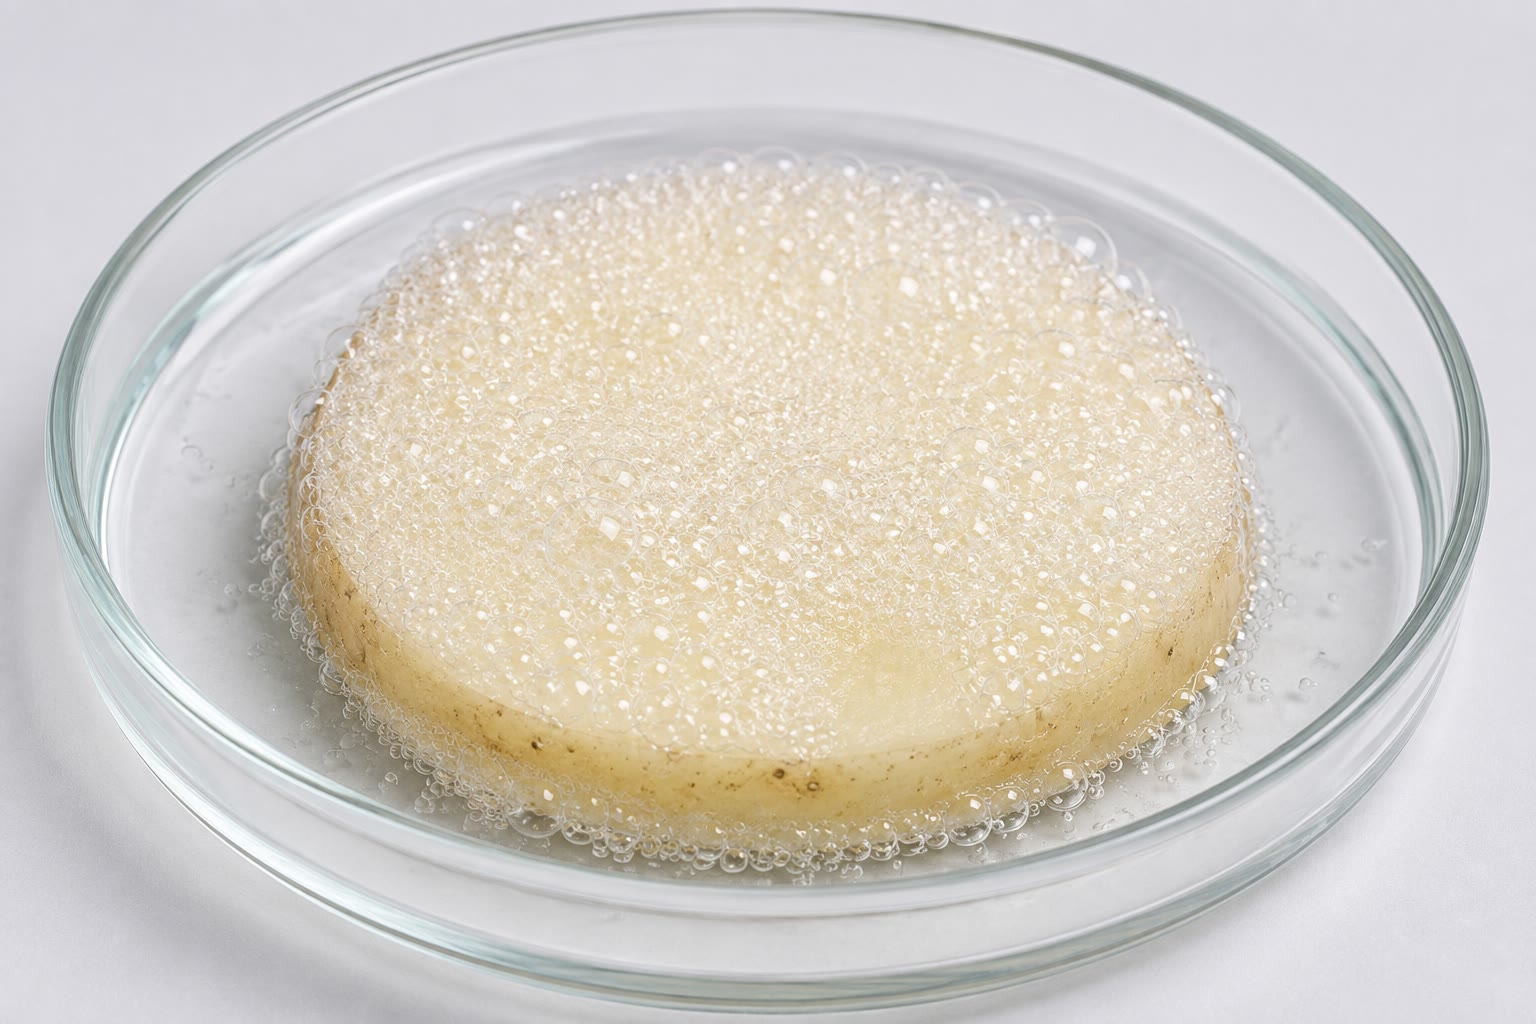
\includegraphics[width=0.5\linewidth]{images/book3/ai/b3-13-catalase-potato.jpg}

{\small Hydrogen peroxide on a cut potato: catalase in the \omterm{def:b1:cell-unit-of-life:cell}{cells}
splits it into water and oxygen forty million times per second per
\omterm{def:b1:enzymes:enzyme}{enzyme} molecule, and the oxygen froths out.}
\end{omfigure}

\begin{proposition}[How the active site works]\label{prop:b1:enzymes:mechanisms}
An \omterm{def:b1:enzymes:enzyme}{active site} accelerates its reaction by several means at once: it
\emph{binds and orients} the \omterm{def:b1:enzymes:enzyme}{substrates} so that the reacting groups
meet in the right geometry, replacing a rare collision by a certain
one; it \emph{strains} the \omterm{def:b1:enzymes:enzyme}{substrate} toward the \omterm{prop:b1:enzymes:whatitdoes}{transition state}
(\emph{induced fit}\index{induced fit}: the \omterm{def:b1:enzymes:enzyme}{enzyme} closes around the
\omterm{def:b1:enzymes:enzyme}{substrate}, and the fit is best for the \omterm{prop:b1:enzymes:whatitdoes}{transition state}); its \omterm{def:b1:proteins:aminoacid}{side
chains} act as \emph{acids and bases}, handing protons to and from the
\omterm{def:b1:enzymes:enzyme}{substrate} at the right moment (histidine, with its p$K_a$ near 7,
does this in many \omterm{def:b1:enzymes:enzyme}{enzymes}); some form a transient \emph{\omterm{def:b1:water-small-molecules:bonds}{covalent
bond}} with the \omterm{def:b1:enzymes:enzyme}{substrate} (serine proteases); and its metal ions
polarise bonds and stabilise charges. Water is largely excluded from
the site, so that charges and \omterm{def:b1:water-small-molecules:water}{hydrogen bonds} act at full strength.
\end{proposition}

\begin{example}[Three enzymes]\label{ex:b1:enzymes:three}
Lysozyme, in tears and egg white, strains a sugar ring of the bacterial
wall into the shape of the \omterm{prop:b1:enzymes:whatitdoes}{transition state} and cuts the chain:
$10^8$-fold acceleration. Carbonic anhydrase, in red \omterm{def:b1:cell-unit-of-life:cell}{cells}, holds a
zinc ion that turns water into a hydroxide poised to attack
$\mathrm{CO_2}$: a million molecules a second, the fastest \omterm{def:b1:enzymes:enzyme}{enzyme}
after catalase. Chymotrypsin, in the pancreatic juice, uses a serine
made reactive by a histidine to cut \omterm{def:b1:proteins:peptide}{proteins} after aromatic residues:
a hundred per second, with a covalent intermediate.
\end{example}

\section{Enzyme kinetics}

\begin{definition}[Initial rate, saturation]\label{def:b1:enzymes:rate}
The \emph{rate}\index{reaction rate} $v$ of an \omterm{def:b1:enzymes:enzyme}{enzyme} reaction is the
amount of product formed per unit time (\unit{mol/s}, or units of
\omterm{def:b1:enzymes:enzyme}{enzyme}: \qty{1}{\micro mol/min}). It is measured as the \emph{initial
rate} $v_0$, before the \omterm{def:b1:enzymes:enzyme}{substrate} is depleted or the product
accumulates. At a fixed \omterm{def:b1:enzymes:enzyme}{enzyme} concentration $v_0$ rises with the
\omterm{def:b1:enzymes:enzyme}{substrate} concentration $[S]$ and then \emph{saturates} at a maximum
$V_{\max}$: the \omterm{def:b1:enzymes:enzyme}{enzyme} is fully occupied and can go no faster.
\end{definition}

\begin{theorem}[Michaelis--Menten]\label{thm:b1:enzymes:mm}
\index{Michaelis--Menten equation}\index{Michaelis constant}
For an \omterm{def:b1:enzymes:enzyme}{enzyme} $E$ that binds its \omterm{def:b1:enzymes:enzyme}{substrate} reversibly and converts it,
\[
E + S \underset{k_{-1}}{\overset{k_1}{\rightleftharpoons}} ES
\overset{k_{\text{cat}}}{\longrightarrow} E + P ,
\]
the initial rate at \omterm{def:b1:enzymes:enzyme}{substrate} concentration $[S]$ is
\[
v_0 = \frac{V_{\max}\,[S]}{K_m + [S]}, \qquad V_{\max} = k_{\text{cat}}\,[E]_{\text{tot}},
\qquad K_m = \frac{k_{-1} + k_{\text{cat}}}{k_1} .
\]
$K_m$, the \emph{\omterm{thm:b1:enzymes:mm}{Michaelis constant}}, is the \omterm{def:b1:enzymes:enzyme}{substrate} concentration
at which the rate is half its maximum, and measures how much \omterm{def:b1:enzymes:enzyme}{substrate}
the \omterm{def:b1:enzymes:enzyme}{enzyme} needs; $k_{\text{cat}}$, the \emph{turnover
number}\index{turnover number}, is the number of \omterm{def:b1:enzymes:enzyme}{substrate} molecules
one \omterm{def:b1:enzymes:enzyme}{enzyme} converts per second when saturated; the ratio
$k_{\text{cat}}/K_m$ is the \emph{catalytic efficiency}, the rate
constant at low \omterm{def:b1:enzymes:enzyme}{substrate}, bounded above by the rate at which
\omterm{def:b1:enzymes:enzyme}{substrate} can reach the \omterm{def:b1:enzymes:enzyme}{enzyme} by diffusion, about
$10^8$--$10^9$ \unit{L.mol^{-1}.s^{-1}}.
\end{theorem}
\begin{proof}
Assume a \emph{steady state} in which $ES$ is formed as fast as it
disappears (valid after the first milliseconds, while $[S] \gg [E]$):
$k_1[E][S] = (k_{-1} + k_{\text{cat}})[ES]$, so $[E][S] = K_m[ES]$
with $K_m$ as defined. Conservation gives $[E] = [E]_{\text{tot}} -
[ES]$; substituting, $([E]_{\text{tot}} - [ES])[S] = K_m[ES]$, hence
$[ES] = [E]_{\text{tot}}[S]/(K_m + [S])$. The rate is
$v_0 = k_{\text{cat}}[ES]$, which gives the formula; at $[S] \gg K_m$,
$v_0 \to k_{\text{cat}}[E]_{\text{tot}} = V_{\max}$, and at $[S] = K_m$,
$v_0 = V_{\max}/2$.
\end{proof}

\begin{omfigure}
\begin{minipage}[b]{0.52\linewidth}\centering
\begin{tikzpicture}
\begin{axis}[
  width=\linewidth, height=5.6cm,
  axis x line=bottom, axis y line=left,
  xmin=0, xmax=22, ymin=0, ymax=1.12,
  xlabel={$[S]$ (\unit{mmol/L})}, ylabel={$v_0$ (\unit{\micro mol/min})},
  xlabel style={font=\small, at={(axis description cs:0.5,-0.14)}, anchor=north},
  ylabel style={font=\small},
  tick label style={font=\small}, xtick={0,5,10,15,20}, ytick={0,0.5,1},
  clip=false,
]
\addplot[very thick, omDef, domain=0:22, samples=100] {x/(2+x)};
\addplot[only marks, mark=*, mark size=1.6pt, omDef!70!black] coordinates {(0.5,0.2) (1,0.333) (2,0.5) (5,0.714) (10,0.833) (20,0.909)};
\draw[dashed, gray] (axis cs:0,1) -- (axis cs:22,1); \node[font=\scriptsize, anchor=south east] at (axis cs:22,1.0) {$V_{\max}$};
\draw[dashed, gray] (axis cs:0,0.5) -- (axis cs:2,0.5) -- (axis cs:2,0); \node[font=\scriptsize, anchor=north] at (axis cs:2,-0.02) {$K_m$};
\end{axis}
\end{tikzpicture}
\end{minipage}\hfill
\begin{minipage}[b]{0.46\linewidth}\centering
\begin{tikzpicture}
\begin{axis}[
  width=\linewidth, height=5.6cm,
  axis x line=middle, axis y line=left,
  xmin=-0.7, xmax=2.2, ymin=0, ymax=5.5,
  xlabel={$1/[S]$}, ylabel={$1/v_0$},
  xlabel style={font=\small, at={(axis description cs:0.5,-0.14)}, anchor=north},
  ylabel style={font=\small},
  tick label style={font=\small}, xtick={0,1,2}, ytick={1,3,5},
  clip=false,
]
\addplot[very thick, omDef, domain=-0.5:2.1, samples=10] {1 + 2*x};
\addplot[only marks, mark=*, mark size=1.6pt, omDef!70!black] coordinates {(2,5) (1,3) (0.5,2) (0.2,1.4) (0.1,1.2) (0.05,1.1)};
\node[font=\scriptsize, anchor=west, align=left] at (axis cs:0.05,4.6) {slope $K_m/V_{\max}$};
\node[font=\scriptsize, anchor=west] at (axis cs:0.05,0.55) {$1/V_{\max}$};
\node[font=\scriptsize, anchor=south] at (axis cs:-0.5,0.1) {$-1/K_m$};
\end{axis}
\end{tikzpicture}
\end{minipage}

{\small Left: the Michaelis--Menten hyperbola for $K_m = \qty{2}{mmol/L}$
and $V_{\max} = \qty{1}{\micro mol/min}$, with the six measured points
of the weekend problem. Right: the same data as a Lineweaver--Burk
plot, $1/v_0$ against $1/[S]$: a straight line whose intercepts give
$V_{\max}$ and $K_m$.}
\end{omfigure}

\begin{method}[Measuring $K_m$ and $V_{\max}$]\label{met:b1:enzymes:lb}
\begin{enumerate}
  \item Prepare a series of \omterm{def:b1:enzymes:enzyme}{substrate} concentrations spanning
        $K_m/4$ to $10K_m$, with the same \omterm{def:b1:enzymes:enzyme}{enzyme} concentration; follow
        the product (colour, absorbance, gas) for the first minute and
        take the slope as $v_0$.
  \item Plot $v_0$ against $[S]$: the hyperbola gives a rough
        $V_{\max}$ (the plateau) and $K_m$ (the concentration at half
        of it).
  \item For precision, invert: $1/v_0 = (K_m/V_{\max})(1/[S]) +
        1/V_{\max}$ (\emph{Lineweaver--Burk}). The line's intercept on
        the $y$ axis is $1/V_{\max}$, on the $x$ axis $-1/K_m$, and its
        slope $K_m/V_{\max}$.
  \item Divide $V_{\max}$ by the \omterm{def:b1:enzymes:enzyme}{enzyme} concentration to get
        $k_{\text{cat}}$; divide by $K_m$ for the efficiency. Repeat
        with an \omterm{def:b1:enzymes:inhibitors}{inhibitor} to see which parameter it changes.
\end{enumerate}
\end{method}

\begin{omfigure}
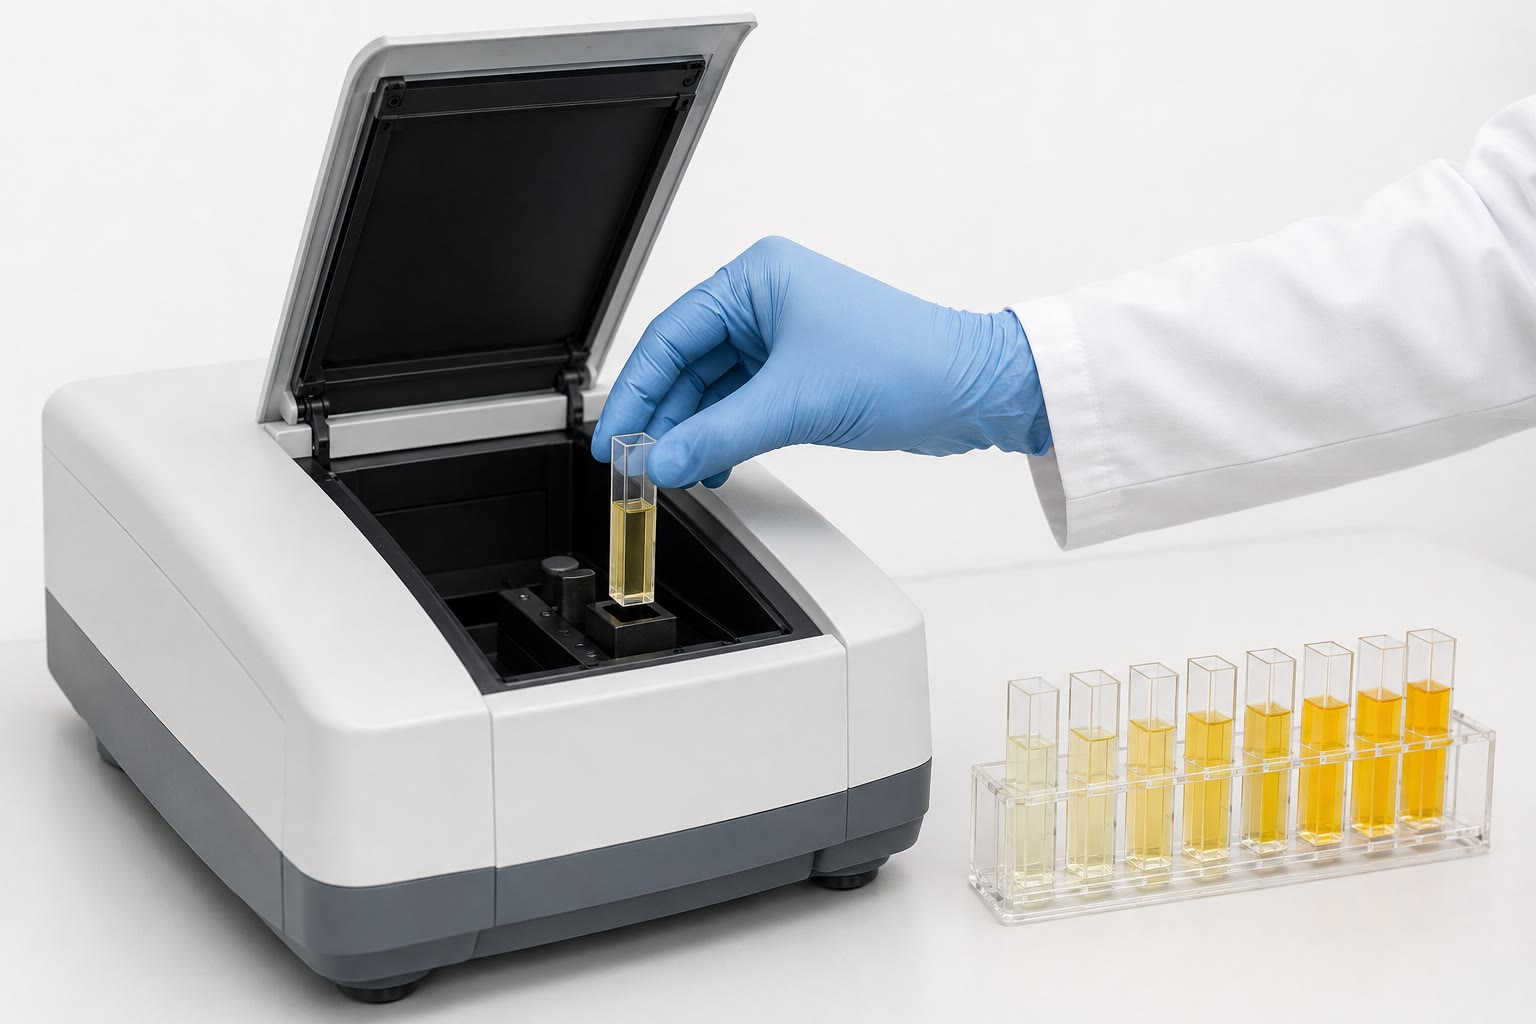
\includegraphics[width=0.5\linewidth]{images/book3/ai/b3-13-spectrophotometer-cuvette.jpg}

{\small An \omterm{def:b1:enzymes:enzyme}{enzyme} assay: the product absorbs light, and the
spectrophotometer records its appearance second by second; the initial
slope is $v_0$.}
\end{omfigure}

\begin{example}[Enzymes compared]\label{ex:b1:enzymes:compare}
\begin{center}
\small
\begin{tabular}{lccc}
\hline
\omterm{def:b1:enzymes:enzyme}{enzyme} & $K_m$ (\unit{mol/L}) & $k_{\text{cat}}$ (\unit{s^{-1}}) & $k_{\text{cat}}/K_m$ (\unit{L.mol^{-1}.s^{-1}}) \\
\hline
catalase & \num{2.5e-2} & \num{4e7} & \num{1.6e9} \\
carbonic anhydrase & \num{1.2e-2} & \num{1e6} & \num{8e7} \\
chymotrypsin & \num{1.5e-2} & 100 & \num{7e3} \\
lysozyme & \num{6e-6} & 0.5 & \num{8e4} \\
\omterm{def:b1:nucleic-acids:chain}{DNA} polymerase & \num{1e-5} & 15 & \num{1.5e6} \\
\hline
\end{tabular}
\end{center}
Catalase and carbonic anhydrase work at the diffusion limit: every
collision with \omterm{def:b1:enzymes:enzyme}{substrate} is productive. Chymotrypsin is slow but
needs to be --- it cuts a \omterm{def:b1:proteins:peptide}{peptide bond}, a far harder job than splitting
peroxide.
\end{example}

\section{Inhibition}

\begin{definition}[Inhibitors]\label{def:b1:enzymes:inhibitors}
An \emph{inhibitor}\index{enzyme inhibitor} lowers the rate of an
\omterm{def:b1:enzymes:enzyme}{enzyme}. \emph{Irreversible} inhibitors bind covalently and destroy the
\omterm{def:b1:enzymes:enzyme}{enzyme}'s activity for good (nerve agents on acetylcholinesterase,
penicillin on the \omterm{def:b1:enzymes:enzyme}{enzyme} that cross-links the bacterial wall, aspirin
on the \omterm{def:b1:enzymes:enzyme}{enzyme} that makes prostaglandins). \emph{Reversible} inhibitors
bind by weak bonds and can be washed away; by where they bind:
\begin{itemize}
  \item \emph{competitive}\index{competitive inhibition}: the inhibitor
        resembles the \omterm{def:b1:enzymes:enzyme}{substrate} and occupies the \omterm{def:b1:enzymes:enzyme}{active site}; it
        raises the apparent $K_m$ (by the factor $1 + [I]/K_i$) and
        \omterm{def:b1:flowering-plant-organization:organs}{leaves} $V_{\max}$ unchanged --- enough \omterm{def:b1:enzymes:enzyme}{substrate} displaces it;
  \item \emph{non-competitive}: the inhibitor binds elsewhere and
        spoils the catalysis whether or not \omterm{def:b1:enzymes:enzyme}{substrate} is bound; it
        lowers $V_{\max}$ and \omterm{def:b1:flowering-plant-organization:organs}{leaves} $K_m$ unchanged --- no amount of
        \omterm{def:b1:enzymes:enzyme}{substrate} overcomes it;
  \item \emph{uncompetitive}: the inhibitor binds only the $ES$
        complex; both $V_{\max}$ and $K_m$ fall.
\end{itemize}
$K_i$, the dissociation constant of the inhibitor, measures its
potency: the lower, the stronger.
\end{definition}

\begin{omfigure}
\begin{tikzpicture}
\begin{axis}[
  width=0.8\linewidth, height=6.0cm,
  axis x line=middle, axis y line=left,
  xmin=-0.8, xmax=2.2, ymin=0, ymax=10.5,
  xlabel={$1/[S]$}, ylabel={$1/v_0$},
  xlabel style={font=\small, at={(axis description cs:0.5,-0.1)}, anchor=north},
  ylabel style={font=\small},
  tick label style={font=\small}, xtick={0,1,2}, ytick={2,4,6,8,10},
  legend style={font=\small, at={(0.03,0.97)}, anchor=north west, draw=none},
  clip=false,
]
\addplot[very thick, omDef, domain=-0.5:2.1, samples=10] {1 + 2*x};
\addlegendentry{no inhibitor}
\addplot[very thick, omThm, domain=-0.25:2.1, samples=10] {1 + 4*x};
\addlegendentry{competitive: same $1/V_{\max}$, steeper}
\addplot[very thick, omProp, domain=-0.5:2.1, samples=10] {2 + 4*x};
\addlegendentry{non-competitive: same $-1/K_m$, higher}
\end{axis}
\end{tikzpicture}

{\small Lineweaver--Burk plots with the two common \omterm{def:b1:enzymes:inhibitors}{inhibitors}. A
competitive \omterm{def:b1:enzymes:inhibitors}{inhibitor} pivots the line about the $y$ intercept
($V_{\max}$ unchanged, $K_m$ raised); a non-competitive one pivots it
about the $x$ intercept ($K_m$ unchanged, $V_{\max}$ lowered).}
\end{omfigure}

\begin{example}[Competition as medicine]\label{ex:b1:enzymes:medicine}
Methanol is harmless until the liver's alcohol dehydrogenase turns it
into formaldehyde and formic acid, which blind and kill. The treatment
is ethanol: a competing \omterm{def:b1:enzymes:enzyme}{substrate} with a lower $K_m$, which keeps the
\omterm{def:b1:enzymes:enzyme}{enzyme} busy while the methanol is excreted unchanged. Statins are
competitive \omterm{def:b1:enzymes:inhibitors}{inhibitors}, resembling the \omterm{prop:b1:enzymes:whatitdoes}{transition state}, of the \omterm{def:b1:enzymes:enzyme}{enzyme}
that commits carbon to \omterm{def:b1:lipids:amphiphilic}{cholesterol}; sulfonamides resemble the
\omterm{def:b1:enzymes:enzyme}{substrate} of a bacterial \omterm{def:b1:enzymes:enzyme}{enzyme} that makes folate, which humans do
not make and so do not miss.
\end{example}

\section{Regulation}

\begin{definition}[Allosteric enzymes]\label{def:b1:enzymes:allosteric}
An \emph{allosteric enzyme}\index{allosteric enzyme} has several
subunits and, besides its \omterm{def:b1:enzymes:enzyme}{active sites}, \emph{regulatory sites} where
effectors bind: \emph{activators} shift it toward its active
conformation, \emph{\omterm{def:b1:enzymes:inhibitors}{inhibitors}} toward the inactive one. Its rate
against $[S]$ is sigmoid, not hyperbolic (\omterm{def:b1:proteins:allostery}{cooperativity} among the
\omterm{def:b1:enzymes:enzyme}{active sites}, as for haemoglobin, \cref{ch:b1:proteins}), so that a
small change of \omterm{def:b1:enzymes:enzyme}{substrate} near the steep part changes the rate
greatly; effectors shift the curve sideways (changing the \omterm{def:b1:enzymes:enzyme}{substrate}
concentration needed) or up and down (changing the maximal rate).
\omterm{def:b1:proteins:allostery}{Allosteric} \omterm{def:b1:enzymes:enzyme}{enzymes} stand at the branch points of metabolism, and the
effectors are the pathway's own products and the \omterm{def:b1:cell-unit-of-life:cell}{cell}'s energy
signals (\omterm{def:b1:water-small-molecules:atp}{ATP}, ADP, AMP).
\end{definition}

\begin{omfigure}
\begin{tikzpicture}
\begin{axis}[
  width=0.86\linewidth, height=6.0cm,
  axis x line=bottom, axis y line=left,
  xmin=0, xmax=10, ymin=0, ymax=1.1,
  xlabel={$[S]$ (relative)}, ylabel={$v_0/V_{\max}$},
  xlabel style={font=\small, at={(axis description cs:0.5,-0.12)}, anchor=north},
  ylabel style={font=\small},
  tick label style={font=\small}, xtick={0,2,4,6,8,10}, ytick={0,0.5,1},
  legend style={font=\small, at={(0.5,-0.22)}, anchor=north, draw=none, legend columns=2, /tikz/every even column/.append style={column sep=0.4cm}},
  clip=false,
]
\addplot[very thick, omDef, domain=0:10, samples=100] {x^3/(3^3+x^3)};
\addlegendentry{allosteric enzyme alone ($n = 3$)}
\addplot[very thick, omExo, domain=0:10, samples=100] {x^3/(1.8^3+x^3)};
\addlegendentry{with an activator: curve shifts left}
\addplot[very thick, omThm, domain=0:10, samples=100] {x^3/(5.5^3+x^3)};
\addlegendentry{with an inhibitor: curve shifts right}
\addplot[thick, dashed, gray, domain=0:10, samples=100] {x/(3+x)};
\addlegendentry{Michaelis--Menten, for comparison}
\draw[dashed, gray] (axis cs:3,0) -- (axis cs:3,0.5);
\end{axis}
\end{tikzpicture}

{\small An \omterm{def:b1:enzymes:allosteric}{allosteric enzyme}. The sigmoid curve makes the rate
sensitive to \omterm{def:b1:enzymes:enzyme}{substrate} near the midpoint; an activator shifts it left
(more active at a given $[S]$), an \omterm{def:b1:enzymes:inhibitors}{inhibitor} right. Near $[S] = 3$
the rate can swing from a tenth to nine tenths of maximum.}
\end{omfigure}

\begin{proposition}[Four ways the cell controls an enzyme]\label{prop:b1:enzymes:control}
\begin{enumerate}
  \item \emph{Feedback inhibition}\index{feedback inhibition}: the end
        product of a pathway is an \omterm{def:b1:proteins:allostery}{allosteric} \omterm{def:b1:enzymes:inhibitors}{inhibitor} of its first
        committed \omterm{def:b1:enzymes:enzyme}{enzyme}, so that the pathway runs only as fast as the
        product is used (isoleucine on threonine deaminase; \omterm{def:b1:water-small-molecules:atp}{ATP} on
        phosphofructokinase, \cref{ch:b1:respiration-fermentation}).
        Response time: milliseconds.
  \item \emph{Covalent modification}\index{covalent modification}:
        a kinase attaches a phosphate to a serine, threonine or
        tyrosine of the \omterm{def:b1:enzymes:enzyme}{enzyme}, a phosphatase removes it, and the two
        forms differ in activity (\omterm{def:b1:carbohydrates:polysaccharide}{glycogen} phosphorylase is switched on
        by phosphorylation, \omterm{def:b1:carbohydrates:polysaccharide}{glycogen} synthase off, by the same
        hormonal signal). Seconds to minutes; reversible; amplifiable
        in cascades.
  \item \emph{Proteolytic activation}: some \omterm{def:b1:enzymes:enzyme}{enzymes} are made as
        inactive precursors (\emph{zymogens}: trypsinogen,
        pepsinogen, the clotting factors) and switched on by cutting
        off a peptide, once and for all, where and when they are
        wanted.
  \item \emph{Amount}: the \omterm{def:b1:cell-unit-of-life:cell}{cell} makes more or less of the \omterm{def:b1:enzymes:enzyme}{enzyme} by
        controlling its gene (\cref{ch:b1:expression-control}) and
        degrades it faster or slower. Minutes to hours.
\end{enumerate}
\end{proposition}

\begin{example}[Isoenzymes]\label{ex:b1:enzymes:isoenzymes}
Lactate dehydrogenase exists in five forms, tetramers of two subunit
types in all combinations; the heart's form has a low $K_m$ for
lactate and is inhibited by pyruvate (it oxidises lactate to feed the
Krebs cycle), the muscle's form has a high $V_{\max}$ and tolerates
pyruvate (it makes lactate in a sprint). The pattern of forms in the
blood reveals which \omterm{def:b1:mammal-organization:organ}{organ} has been damaged --- a heart attack releases
the heart's.
\end{example}

\section{Temperature and pH}

\begin{proposition}[Enzymes and their environment]\label{prop:b1:enzymes:environment}
The rate of an \omterm{def:b1:enzymes:enzyme}{enzyme} reaction roughly doubles for every
\qty{10}{\celsius} ($Q_{10} \approx 2$) as thermal energy carries more
molecules over the barrier, until the \omterm{def:b1:enzymes:enzyme}{enzyme} begins to unfold
(\qtyrange{40}{60}{\celsius} for most; \qty{100}{\celsius} for the
\omterm{def:b1:enzymes:enzyme}{enzymes} of hot-spring bacteria) and the rate collapses. Each \omterm{def:b1:enzymes:enzyme}{enzyme} has
a \emph{pH optimum}, where the ionisation of its catalytic residues
and of its \omterm{def:b1:enzymes:enzyme}{substrate} is right: pepsin, in the stomach, near pH 2;
trypsin, in the intestine, near 8; most intracellular \omterm{def:b1:enzymes:enzyme}{enzymes} near 7.
Away from the optimum the rate falls, and far from it the \omterm{def:b1:proteins:peptide}{protein}
denatures. Temperature and pH act on the \omterm{def:b1:proteins:peptide}{protein}; the \omterm{def:b1:cell-unit-of-life:cell}{cell} keeps both
within the range where its thousand \omterm{def:b1:enzymes:enzyme}{enzymes} all work.
\end{proposition}

\begin{example}[A fever and a hot spring]\label{ex:b1:enzymes:fever}
A fever of \qty{40}{\celsius} speeds every reaction of the body by a
quarter and begins to unfold the most fragile \omterm{def:b1:proteins:peptide}{proteins}; at
\qty{42}{\celsius} the brain's fail. The \omterm{def:b1:nucleic-acids:chain}{DNA} polymerase of a bacterium
from a \qty{75}{\celsius} spring survives \qty{95}{\celsius}, which is
why it can be cycled through the melting of \omterm{def:b1:nucleic-acids:chain}{DNA} thousands of times
and became the \omterm{def:b1:enzymes:enzyme}{enzyme} of the polymerase chain reaction (the Year 3
volume): thermostability is a property of the sequence, not of the
chemistry catalysed.
\end{example}

\section{Exercises}

\begin{exercise}[$\star$]\label{exo:b1:enzymes:1}
What does an \omterm{def:b1:enzymes:enzyme}{enzyme} change in a reaction, and what does it leave
unchanged? Illustrate with the energy profile.
\end{exercise}

\begin{exercise}[$\star$]\label{exo:b1:enzymes:2}
Define $K_m$, $V_{\max}$, $k_{\text{cat}}$ and $k_{\text{cat}}/K_m$,
with units.
\end{exercise}

\begin{exercise}[$\star$]\label{exo:b1:enzymes:3}
From the Lineweaver--Burk figure of the \omterm{def:b1:enzymes:inhibitors}{inhibitors}, read $V_{\max}$
and $K_m$ for the uninhibited \omterm{def:b1:enzymes:enzyme}{enzyme} and for each \omterm{def:b1:enzymes:inhibitors}{inhibitor}.
\end{exercise}

\begin{exercise}[$\star$]\label{exo:b1:enzymes:4}
Name the four ways a \omterm{def:b1:cell-unit-of-life:cell}{cell} regulates an \omterm{def:b1:enzymes:enzyme}{enzyme}'s activity and give
the timescale of each.
\end{exercise}

\begin{exercise}[$\star\star$]\label{exo:b1:enzymes:5}
An \omterm{def:b1:enzymes:enzyme}{enzyme} has $K_m = \qty{0.1}{mmol/L}$ and $V_{\max} =
\qty{50}{\micro mol/min}$. Compute $v_0$ at $[S] = 0.02$, $0.1$, $1$
and \qty{10}{mmol/L}. At what $[S]$ is $v_0 = 0.9\,V_{\max}$?
\end{exercise}

\begin{exercise}[$\star\star$]\label{exo:b1:enzymes:6}
Lowering $E_a$ by \qty{20}{kJ/mol} at \qty{37}{\celsius} multiplies
the rate by what factor? By how much must $E_a$ fall to gain a factor
$10^{10}$?
\end{exercise}

\begin{exercise}[$\star\star$]\label{exo:b1:enzymes:7}
$\qty{2}{pmol}$ of carbonic anhydrase in \qty{1}{mL} gives
$V_{\max} = \qty{120}{mmol/L}$ per minute. Compute $k_{\text{cat}}$
and, with $K_m = \qty{12}{mmol/L}$, the efficiency. Compare with the
diffusion limit.
\end{exercise}

\begin{exercise}[$\star\star$]\label{exo:b1:enzymes:8}
A competitive \omterm{def:b1:enzymes:inhibitors}{inhibitor} at \qty{2}{mmol/L} doubles the apparent $K_m$.
Compute $K_i$. What \omterm{def:b1:enzymes:enzyme}{substrate} concentration restores the rate to
\qty{90}{\%} of $V_{\max}$ with and without the \omterm{def:b1:enzymes:inhibitors}{inhibitor}, if
$K_m = \qty{1}{mmol/L}$?
\end{exercise}

\begin{exercise}[$\star\star$]\label{exo:b1:enzymes:9}
Explain why \omterm{prop:b1:enzymes:control}{feedback inhibition} acts on the first committed step of a
pathway rather than the last, and why the \omterm{def:b1:enzymes:inhibitors}{inhibitor} is usually the
end product rather than an intermediate.
\end{exercise}

\begin{exercise}[$\star\star\star$]\label{exo:b1:enzymes:10}
Trypsinogen is activated in the intestine, not in the pancreas that
makes it; a small fraction activated early destroys the pancreas.
Explain the logic of zymogens, the role of the \omterm{def:b1:enzymes:enzyme}{enzyme} that activates
trypsinogen, and why the pancreas also makes a trypsin \omterm{def:b1:enzymes:inhibitors}{inhibitor}.
\end{exercise}

\begin{exercise}[$\star\star\star$]\label{exo:b1:enzymes:11}
An \omterm{def:b1:enzymes:allosteric}{allosteric enzyme} with $n = 3$ and half-saturation at $[S]_{0.5}
= 3$ has its curve shifted to $[S]_{0.5} = 5.5$ by an \omterm{def:b1:enzymes:inhibitors}{inhibitor}.
Compute the rate at $[S] = 3$ with and without the \omterm{def:b1:enzymes:inhibitors}{inhibitor}, and
compare with the change a competitive \omterm{def:b1:enzymes:inhibitors}{inhibitor} of the same
$K_m$-shift would produce on a Michaelis--Menten \omterm{def:b1:enzymes:enzyme}{enzyme}. What does
\omterm{def:b1:proteins:allostery}{cooperativity} add to regulation?
\end{exercise}

\begin{exercise}[$\star\star\star$]\label{exo:b1:enzymes:12}
``An \omterm{def:b1:enzymes:enzyme}{enzyme} is a catalyst that has been told what to do.'' Discuss in a
paragraph: catalysis versus specificity, regulation as the added
information, and the cost of a regulated \omterm{def:b1:enzymes:enzyme}{enzyme} compared with a bare
catalyst.
\end{exercise}

\section{Problem: An Enzyme Measured}

\begin{problem}[{Weekend problem --- an esterase assayed at six
\omterm{def:b1:enzymes:enzyme}{substrate} concentrations, alone and with two \omterm{def:b1:enzymes:inhibitors}{inhibitors}, its constants
extracted and its behaviour in the \omterm{def:b1:cell-unit-of-life:cell}{cell} predicted, ending on its $K_m$,
$V_{\max}$ and $K_i$}]
\label{pb:b1:enzymes:1}
An esterase is assayed in \qty{1.0}{mL} at \qty{25}{\celsius}, pH 7.5,
with \qty{10}{nmol/L} of \omterm{def:b1:enzymes:enzyme}{enzyme}. The initial rates (\unit{\micro mol/min})
at six \omterm{def:b1:enzymes:enzyme}{substrate} concentrations, alone and in the presence of
\qty{1.0}{mmol/L} of \omterm{def:b1:enzymes:inhibitors}{inhibitor} I or \qty{1.0}{mmol/L} of \omterm{def:b1:enzymes:inhibitors}{inhibitor} J:

\begin{center}
\small
\begin{tabular}{lcccccc}
\hline
$[S]$ (\unit{mmol/L}) & 0.5 & 1 & 2 & 5 & 10 & 20 \\
\hline
$v_0$, no \omterm{def:b1:enzymes:inhibitors}{inhibitor} & 0.200 & 0.333 & 0.500 & 0.714 & 0.833 & 0.909 \\
$v_0$, with I & 0.111 & 0.200 & 0.333 & 0.556 & 0.714 & 0.833 \\
$v_0$, with J & 0.100 & 0.167 & 0.250 & 0.357 & 0.417 & 0.455 \\
\hline
\end{tabular}
\end{center}

\medskip
\noindent\textbf{Part I --- The \omterm{def:b1:enzymes:enzyme}{enzyme} alone.}
\begin{enumerate}
  \item Compute $1/[S]$ and $1/v_0$ for the six points without
        \omterm{def:b1:enzymes:inhibitors}{inhibitor}.
  \item Show that the points lie on a straight line and find its
        slope and intercept.
  \item Deduce $V_{\max}$ and $K_m$.
  \item Verify with the \omterm{thm:b1:enzymes:mm}{Michaelis--Menten equation} at $[S] =
        \qty{5}{mmol/L}$.
  \item Compute the amount of \omterm{def:b1:enzymes:enzyme}{enzyme} in the assay (moles) and
        $k_{\text{cat}}$ in \unit{s^{-1}}.
  \item Compute $k_{\text{cat}}/K_m$ and compare with the diffusion
        limit.
  \item At what \omterm{def:b1:enzymes:enzyme}{substrate} concentration is the \omterm{def:b1:enzymes:enzyme}{enzyme} working at
        \qty{95}{\%} of $V_{\max}$?
\end{enumerate}

\medskip
\noindent\textbf{Part II --- \omterm{def:b1:enzymes:inhibitors}{Inhibitor} I.}
\begin{enumerate}[resume]
  \item Compute $1/v_0$ for the six points with I and find the slope
        and intercept of their line.
  \item Deduce the apparent $V_{\max}$ and $K_m$ with I.
  \item Which parameter changed? Classify the \omterm{def:b1:enzymes:inhibitors}{inhibitor}.
  \item Compute $K_i$ from $K_m^{\text{app}} = K_m(1 + [I]/K_i)$.
  \item At $[S] = \qty{2}{mmol/L}$, what concentration of I halves the
        rate? At $[S] = \qty{20}{mmol/L}$?
  \item Propose what I might be, structurally, and where it binds.
\end{enumerate}

\medskip
\noindent\textbf{Part III --- \omterm{def:b1:enzymes:inhibitors}{Inhibitor} J.}
\begin{enumerate}[resume]
  \item Compute the slope and intercept of the line with J and deduce
        the apparent $V_{\max}$ and $K_m$.
  \item Classify J and compute its $K_i$ from $V_{\max}^{\text{app}} =
        V_{\max}/(1 + [J]/K_i)$.
  \item Explain why raising the \omterm{def:b1:enzymes:enzyme}{substrate} cannot overcome J.
  \item Doubling the \omterm{def:b1:enzymes:enzyme}{enzyme} concentration in the presence of J does
        what to the rate? And in the presence of I?
\end{enumerate}

\medskip
\noindent\textbf{Part IV --- In the \omterm{def:b1:cell-unit-of-life:cell}{cell}.}
The \omterm{def:b1:cell-unit-of-life:cell}{cell} holds the \omterm{def:b1:enzymes:enzyme}{substrate} at \qty{0.5}{mmol/L} and the \omterm{def:b1:enzymes:enzyme}{enzyme} at
\qty{10}{nmol/L} in a volume of \qty{1000}{\micro m^3}, at
\qty{37}{\celsius}, with $Q_{10} = 2$.
\begin{enumerate}[resume]
  \item Compute the rate in the \omterm{def:b1:cell-unit-of-life:cell}{cell} (molecules of product per second
        in the whole \omterm{def:b1:cell-unit-of-life:cell}{cell}).
  \item The product is needed at \qty{3e6}{} molecules per second.
        By what factor must the \omterm{def:b1:cell-unit-of-life:cell}{cell} raise the rate, and name two ways
        it could.
  \item The product is a competitive \omterm{def:b1:enzymes:inhibitors}{inhibitor} of the \omterm{def:b1:enzymes:enzyme}{enzyme} with
        $K_i = \qty{0.2}{mmol/L}$, and accumulates to
        \qty{0.4}{mmol/L}. Compute the rate then, and comment on what
        this achieves.
  \item The \omterm{def:b1:enzymes:enzyme}{enzyme} is phosphorylated by a kinase, which lowers its
        $K_m$ to \qty{0.4}{mmol/L}. Compute the rate at
        \qty{0.5}{mmol/L} of \omterm{def:b1:enzymes:enzyme}{substrate} before and after.
  \item The \omterm{def:b1:enzymes:enzyme}{enzyme}'s pH optimum is 7.5 and its activity halves at pH
        6.5. A \omterm{def:b1:eukaryotic-cell:endomembrane}{lysosome} is at pH 5. Predict, qualitatively, its
        activity there and explain in terms of ionisable residues.
  \item A mutation replaces the histidine of the \omterm{def:b1:enzymes:enzyme}{active site} by
        alanine. Predict the effect on $K_m$ and on $k_{\text{cat}}$,
        with a reason for each.
  \item Explain why the \omterm{def:b1:cell-unit-of-life:cell}{cell} keeps the \omterm{def:b1:enzymes:enzyme}{substrate} near $K_m$ rather
        than far above it.
  \item State the result: $K_m$, $V_{\max}$, $k_{\text{cat}}$ of the
        esterase, the type and $K_i$ of each \omterm{def:b1:enzymes:inhibitors}{inhibitor}.
\end{enumerate}
\end{problem}
